%!TEX root = ../../super_main.tex

\chapter{Quality Assurance}
\label{cha:quality_assurance}

\todo{Overvej at skrive kort om pair programming}

\section{Automated Unit Test}
\label{sec:automated_unit_test}

\section{Continuous Integration}
\label{sec:continuous_integration}
As mentioned in \secref{sec:extreme_programming}, we wanted a continuous integration server in order to ensure that our code base always was at a stable state. We installed Jenkins on the same server that makes up the server part of our client-server architecture because it was easily available. Jenkins is an open source automation server, which supports various different plugins that helps with builds, viewing test results, etc. We configured this Jenkins server to be notified whenever our Github version control code repositories for both Android and PHP code were changed. When this notification happened, Jenkins would build the corresponding project and run its tests. Whenever the build projects would go from a previously successful build to a now failing build or vice versa, the Jenkins system would send out mails to our group, so we were aware that something went wrong or that it was now fixed again. This made it possible for us to give immediate attention to issues that we did not catch before pushing our content to the version control. See \figref{fig:jenkins_front_page} for an illustration of how the front page of Jenkins. In the left side, the build queue can be seen, which shows if any builds are currently running. In the center, the various projects that are currently configured for the Jenkins setup can be seen. The blue circle changes to red if the most recent build was a failure, and besides that, it can be seen how long time has passed since the most recent pass, most recent failure, and how long the last build took to finish.  

\begin{figure}[!htbp]
    \centering
    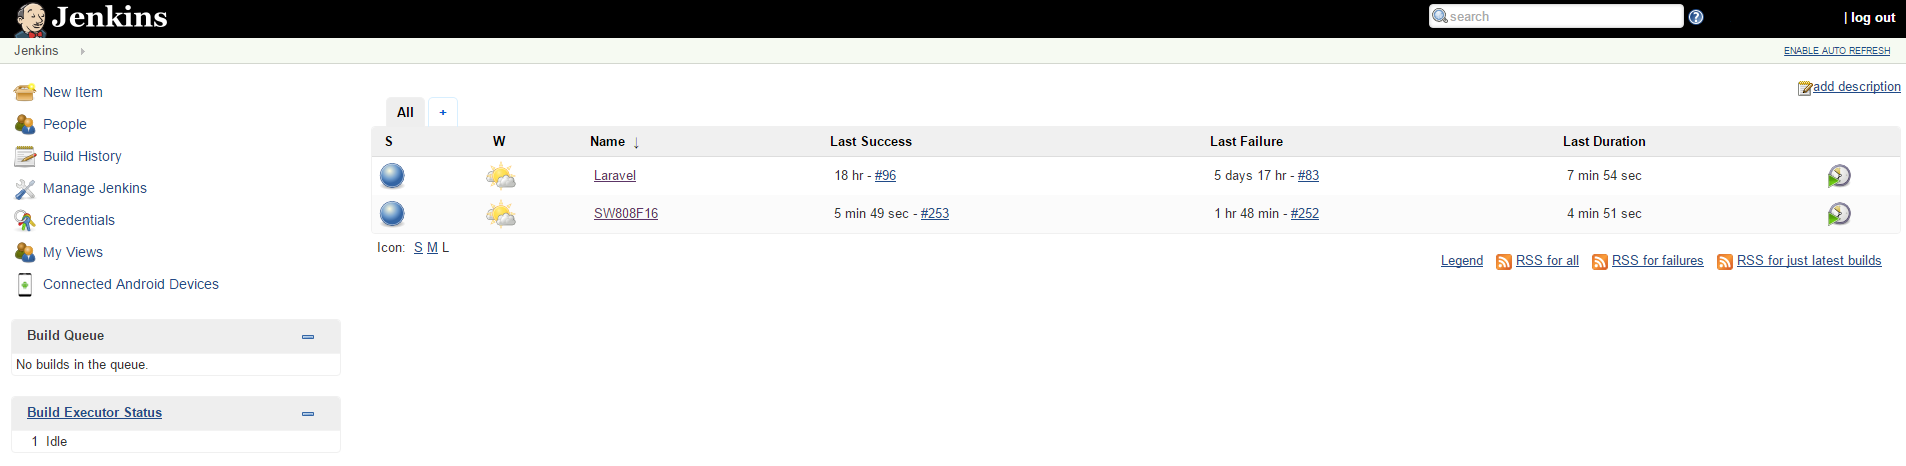
\includegraphics[width=\textwidth]{graphic/quality_assurance/jenkins_frontpage.png}
    \caption{Jenkins CI front page}
    \label{fig:jenkins_front_page}
\end{figure}

\section{Monkey Test}
\label{sec:monkey_test}

\section{Configuration Test}
\label{sec:configuration_test}

\section{Pair Review}
\label{sec:pair_review}


